%!TEX root = ../masters_thesis.tex

\chapter{Concept} % (fold)
\label{cha:concept}

The first section of this chapter explains the spatio-temporal data model developed in this thesis and the related concepts of an  \emph{Hivent} and an \emph{Area}. It shows ten \emph{Historical Geographic Operations} that represent all kinds of changes that can happen in the development of a country. The second section introduces \emph{HistoGlobe}, the application used in this thesis. The chapter finishes with the \emph{EditMode} and the \emph{HistoGraph} as interface extensions to HistoGlobe to visualize and edit historical changes of countries.

% - - - - - - - - - - - - - - - - - - - - - - - - - - - - - - - - - - - - - - -
\paragraph{Area identity} % (fold)
\label{par:area_identity}

Given the example of Germany, the Area is independent from both its territory and short name: In 1949, four years after the end of World War II, the German Democratic Republic (\emph{East Germany}) and the Federal Republic of Germany (\emph{West Germany}) were created. In 1957, the Saar Protectorate (\emph{Saarland}) joined West Germany. Although the territory of the Area has changed, it is still the same Area. In 1990, East and West Germany reunited to what is currently known as Germany. This Germany is still the Federal Republic of Germany, so it is juristically the same as West Germany before 1990. That means that also the short name of an Area can change (West Germany to Germany) without affecting the identity of the Area.


% paragraph area_identity (end)

% - - - - - - - - - - - - - - - - - - - - - - - - - - - - - - - - - - - - - - -
\paragraph{Historical Geographic Operations} % (fold)
\label{par:historical_geographic_operations}


\begin{enumerate}

  \item Identity-changing operations for one Area
  \begin{description}
    \item[CRE -- Creation]
    A new Area is created with a new name and a new territory fully on previously unclaimed land. \\
    \begin{footnotesize}
      The Roman Kingdom (753 - 509 B.C.) was created in Latinum, today central Italy, in a region that did not have anything before which would be considered a political entity.
    \end{footnotesize}
    \item[ICH -- Identity Change]
    The formal name of an Area changes, therefore the old Area is destructed and a new Area with the same territory is created. The old Area is the historical predecessor of the new Area. \\
    \begin{footnotesize}
      In the end of the Cold War, the Polish People's Republic (1952-1989) got renamed to present-day Republic of Poland (since 1989). Although the short name (Poland) stayed, the new country is a new political entity and is therefore to be modeled a new Area.
    \end{footnotesize}
    \item[CES -- Cessation]
    An Area stops to exist and ceases, leaving unclaimed land. Cessation is the inverse operation of Creation. \\
    \begin{footnotesize}
      The Minoan civilisation, populating the nowadays Greek island of Crete (3650 to 1400 B.C.) declined and left no immediate successor.
    \end{footnotesize}
  \end{description}

  \item Identity-changing operations for two or more Area
  \begin{description}
    \item[UNI -- Unification]
    Two or more old Areas unify to a new Area. The old Areas cease, becoming the historical predecessors of the new Area. It receives a new name and its is the union of the territories of the old Areas. \\
    \begin{footnotesize}
      In 1922, the Russian SFSR, the Transcaucasian SFSR, the Ukrainian SSR and the Byelorussian SSR unified and formed the Union of Soviet Socialist Republics (USSR).
    \end{footnotesize}
    \item[INC -- Incorporation]
    One or more old Areas are incorporated into another Area. This areas preserves its identity, i.e. formal name, but may get a new short name. Its territory in enlarged by the union of the old Areas. The old Areas are historical predecessors of the new Area. \\
    \begin{footnotesize}
      In 1990, the territory of the German Democratic Republic (East Germany) became part of the Federal Republic of Germany (West Germany). Although this event is known as the \emph{German Reunification}, it is historically an incorporation of East Germany into West Germany \cite{incorporationEastWestGermany}. Additionally, the commonly known short name of West Germany got changed into Germany, creating the country existing until today.
    \end{footnotesize}
    \item[SEP -- Separation]
    As the inverse of unification, one old Area is preceded by two or more new Areas. Each new Area gets a new name, receives a part of the territory of the old Area, and the old Area as the historical predecessor. \\
    \begin{footnotesize}
      In 1993, the Czech and Slovak Federal Republic, commonly known as Czechoslovakia, dissolved into present-day Czech Republic and Solvak Republic, creating two new countries.
    \end{footnotesize}
    \item[SEC -- Secession]
    As the inverse of incorporation, one or more new areas are ceded from a previously exising area. This Area may receive a new short name, but keeps its formal name and therefore its identity. Each new Area gets a new name, receives the previously existing Area as the historical predecessor and a part of its territory. \\
    \begin{footnotesize}
      In 2008, the Republic of Kosovo declared independence from Serbia and has since then partially received international recognition, so it can be seen as a new country. Unlike in the case of separation, Serbia kept its name, but ceded only a part of its territory to Kosovo. Therefore, Serbia kept its identity and keeps on existing.
    \end{footnotesize}
  \end{description}

  \item Identity-preserving operations for one or more Areas
  \begin{description}
    \item[BCH -- Border Change]
    Parts of the territory of one Area is ceded to one of its neighors. Therefore, the border shared by two neighboring Areas changes. The names of the two Areas remain unchanged. Geographically, this operation preserves also the topology: Since only the border between two countries changes, they are still neighboring like before. \\
    \begin{footnotesize}
      As the result of the Treaty of Versailles in 1919, the German Empire ceded 13 \% of its territory, e.g. Alsace-Lorraine to France, changing the German-French border.
    \end{footnotesize}
    \item[TCH -- Territory Change]
    A territory change is a special case of a border change: The territory of an Area is partially expanding into previously unclaimed land or partially shrinking, leaving unclaimed land. \\
    \begin{footnotesize}
      Throughout the British Colonization of North America, several settlements and later colonies, e.g. in 1607 the colony of Virginia, were found. Their territory was often expanded westwards, incorporating previously unclaimed land.
    \end{footnotesize}
    \item[NCH -- Name Change]
    An Area changes its short name. Its territory, formal name and identity is preserved. \\
    \begin{footnotesize}
      The most recent geopolitical change happened on 5. May 2016, when the cabinet of Czech Republic approved that the country will now offically be called ``Czechia''. However, the formal name stays Czech Republic.
    \end{footnotesize}
  \end{description}
\end{enumerate}

\begin{table}[!h]
\begin{center}
\begin{tabular}{m{0.65cm} m{2.5cm} m{2.2cm}
                m{0.35cm} m{0.35cm} m{0.35cm} m{0.01cm}
                m{0.35cm} m{0.3cm} m{0.35cm} m{0.01cm}
                m{0.35cm} m{0.3cm} m{0.88cm}}
  \toprule
    \multicolumn{2}{c}{operation}
  & visualization
  & \multicolumn{e3}{c}{Area change} &
  & \multicolumn{3}{c}{name change} &
  & \multicolumn{3}{c}{territory change} \\
  & & &
  old & $ \leftrightarrow_H $ & new & &
  old & $ \rightarrow $ & new & &
  old & $ \rightarrow $ & new \\

  \midrule[0.07em]
  \texttt{CRE} & Creation & 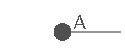
\includegraphics{graphics/concept/operations/CRE} &
  $ \emptyset $ & $ \rightarrow $ & $ A $ & &
  $ \emptyset $ & $ \rightarrow $ & $ A_N $ & &
  $ \emptyset $ & $ \rightarrow $ & $ A_T $ \\

  \midrule[0.01em]
  \texttt{ICH} & Identity Change & 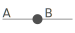
\includegraphics{graphics/concept/operations/ICH} &
  $ A   $ & $ \leftrightarrow_H $ & $ B $ & &
  $ A_N $ & $ \rightarrow $       & $ B_N $ & &
  $ A_T $ & $ \rightarrow $       & $ B_T $ \\

  \midrule[0.01em]
  \texttt{CES} & Cessation & 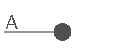
\includegraphics{graphics/concept/operations/CES} &
  $ A $   & $ \rightarrow $       & $ \emptyset $ & &
  $ A_N $ & $ \rightarrow $       & $ \emptyset $ & &
  $ A_T $ & $ \rightarrow $       & $ \emptyset $ \\

  \midrule[0.07em]
  \multirow{3}{*}{\texttt{UNI}} &
  \multirow{3}{*}{Unification} &
  \multirow{3}{*}{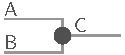
\includegraphics{graphics/concept/operations/UNI}} &
  $ A $   & $ \leftrightarrow_H $ & $ C $ & &
  $ A_N $ & $ \rightarrow $       & $ \emptyset $ & &
  $ A_T $ & $ \rightarrow $       & $ \emptyset $ \\
  & & &
  $ B $   & $ \leftrightarrow_H $ & $ C $ & &
  $ B_N $ & $ \rightarrow $       & $ \emptyset $ & &
  $ B_T $ & $ \rightarrow $       & $ \emptyset $ \\
  & & &
  & & & &
  $ \emptyset $ & $ \rightarrow $ & $ C_N $ & &
  $ \emptyset $ & $ \rightarrow $ & $ C_T $ \footnotemark \\

  \midrule[0.01em]
  \multirow{2}{*}{\texttt{INC}} &
  \multirow{2}{*}{Incorporation} &
  \multirow{2}{*}{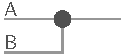
\includegraphics{graphics/concept/operations/INC}} &
  & & & &
  $ (A_N $ & $ \rightarrow $      & $ A_{N'}) $ & &
  $ A_T $ & $ \rightarrow $       & $ A_{T'} $ \footnotemark \\
  & & &
  $ B $   & $ \leftrightarrow_H $ & $ A $ & &
  $ B_N $ & $ \rightarrow $       & $ \emptyset $ & &
  $ B_T $ & $ \rightarrow $       & $ \emptyset $ \\

  \midrule[0.01em]
  \multirow{3}{*}{\texttt{SEP}} &
  \multirow{3}{*}{Separation} &
  \multirow{3}{*}{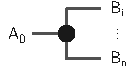
\includegraphics{graphics/concept/operations/SEP}} &
  $ A $         & $ \leftrightarrow_H $ & $ B $ & &
  $ A_N $       & $ \rightarrow $       & $ \emptyset $ & &
  $ A_T $       & $ \rightarrow $       & $ \emptyset $ \\
  & & &
  $ A $         & $ \leftrightarrow_H $ & $ C $ & &
  $ \emptyset $ & $ \rightarrow $       & $ B_N $ & &
  $ \emptyset $ & $ \rightarrow $       & $ B_T $ \\
  & & &
  & & & &
  $ \emptyset $ & $ \rightarrow $       & $ C_N $ & &
  $ \emptyset $ & $ \rightarrow $       & $ C_T $ \footnotemark \\

  \midrule[0.01em]
  \multirow{2}{*}{\texttt{SEC}} &
  \multirow{2}{*}{Secession} &
  \multirow{2}{*}{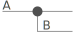
\includegraphics{graphics/concept/operations/SEC}} &
  $ A $     & $ \leftrightarrow_H $     & $ B $ & &
  $ (A_N $  & $ \rightarrow $           & $ A_{N'}) $ & &
  $ A_T $   & $ \rightarrow $           & $ A_{T'} $ \\
  & & &
  & & & &
  $ \emptyset $ & $ \rightarrow $ & $ B_N $ & &
  $ \emptyset $ & $ \rightarrow $ & $ B_T $ \footnotemark \\

  \midrule[0.07em]
  \multirow{1}{*}{\texttt{NCH}} &
  \multirow{1}{*}{Name Change} &
  \multirow{1}{*}{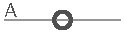
\includegraphics{graphics/concept/operations/NCH_TCH}} &
  & & & &
  $ A_N $ & $ \rightarrow $ & $ A_{N'} $ & &
  & & \\

  \midrule[0.01em]
  \multirow{2}{*}{\texttt{BCH}} &
  \multirow{2}{*}{Border Change} &
  \multirow{2}{*}{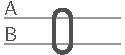
\includegraphics{graphics/concept/operations/BCH}} &
  & & & &
  & & & &
  $ A_T $ & $ \rightarrow $ & $ A_{T'} $ \\
  & & &
  & & & &
  & & & &
  $ B_T $ & $ \rightarrow $ & $ B_{T'} $ \footnotemark \\

  \midrule[0.01em]
  \multirow{1}{*}{\texttt{TCH}} &
  \multirow{1}{*}{Territory Change} &
  \multirow{1}{*}{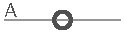
\includegraphics{graphics/concept/operations/NCH_TCH}} &
  & & & &
  & & & &
  $ A_T $ & $ \rightarrow $ & $ A_{T'} $ \\

  \bottomrule
\end{tabular}
\caption{Overview about all 10 historical geographic operations}
\small{$A \leftrightarrow_H B$ denotes historical relationship between two Areas, \\ i.e. $A$ is predecessor of $B$ and $B$ is successor of $A$}
\label{tab:historical_geographic_operations}
\end{center}
\end{table}

\addtocounter{footnote}{-4}
\footnotetext{$C_{T} = A_T \cup B_T$}
\addtocounter{footnote}{1}
\footnotetext{$A_{T'} = A_T \cup B_T$}
\addtocounter{footnote}{1}
\footnotetext{$B_T \cup C_{T} = A_T$}
\addtocounter{footnote}{1}
\footnotetext{$A_{T'} \cup B_{T} = A_T$}
\addtocounter{footnote}{1}
\footnotetext{$A_{T} \cup B_{T} = A_{T'} \cup B_{T'}$}

% paragraph historical_geographic_operations (end)


% - - - - - - - - - - - - - - - - - - - - - - - - - - - - - - - - - - - - - - -

% subsection historical_changes (end)

% ------------------------------------------------------------------------------
\subsection{Four-Domain Model} % (fold)
\label{sub:four_domain_model}

According to the extension of the Three Domain model (see section \ref{sub:three_domain_model}), a spatio-temporal object can be represented separetely in the spatial, temporal and thematic domain. Additionally, the semantic domain uniquely identifies an object and is invariant. This applies to the concept of an Area that represents a country.

id: formal name

semantic: id (formal name)
spatial:  spatial attributes (territory)
temporal: Hivent -> HistoricalChange -> AreaChange
thematic: aspatial attributes (short name)

Since the data model uses the concept of several existing one, it will derive also its name from it: The Hivent-Based Three-Domain Spatio-Temporal History Graph Data Model for Time-Stamped Vector Geometry
... or in short: HBTDSTHGDMTSVG

% subsection four_domain_model (end)